\documentclass{article}
\usepackage{graphicx} % Required for inserting images
\usepackage{hyperref}
\usepackage{caption}
\usepackage{subcaption}

\title{On Image Compression: Fourier and Wavelet Transforms}
\author{ \\ Abdelrahman Abdelghany - 202301000 \\ \\ Yehia Saied - 202301237 \\ \\ Martin Rober - 202301070 \\ \\ Mostafa Mahmoud - 20230905 \\ \\ Mohamed Hossam \\ \\ \\ \\ \\  }
\date{December 30th, 2024}

\begin{document}

\maketitle

\newpage
\section*{Abstract}
The Fourier Transform, first introduced by Jean-Baptiste Joseph Fourier in 1822 to solve heat diffusion problems, 
is a mathematical tool mainly used to segregate the frequencies composing a function, allowing its swift analysis 
into a frequency spectrum. It is utilized in the modern day almost routinely, from detecting the seismic activity 
induced by explosives from across the globe, to its indispensable use in signal analysis, all the way to image 
compression. The latter of which we will be exploring.

Image compression, whether lossy or lossless, is the act of reducing the data present within an image file in order 
to reduce its size. Lossy image compression does so at the cost of quality, which can sometimes be beneficial in 
cases where space is prioritized over fidelity. For cases where lossy compression is concerned, the Fourier 
Transform may be used in order to transform the image into a new domain, where the fine details of the image 
can be excised, before transforming back and obtaining a less-crisp, but more memory-efficient image file.

\newpage
\section*{Fourier Transform: What?}
The Fourier Transform is a mathematical tool with many uses. Synonymous with signals, it is a tool which 
utilizes the special quality of trigonometric functions, in that they are orthogonal (and form a basis) in 
order to project any function into a linear combination of said basis, essentially allowing the analysis of
any function (continuous or not) into a weighted sum of pure frequencies.
\newline \newline
The Fourier Transform is given by
$$\hat{f}(\zeta) = \langle f(t), e^{-2\pi i \zeta t} \rangle = \int_{-\infty}^{\infty} f(t) e^{-2\pi i \zeta t} dt$$
It is essentially the inner product of the function to be analyzed and the complex exponential.
\section*{Fourier Transform: How?}
We've discussed what a Fourier Transform is. However, how does it actually work?
\newline \newline
The answer to that question is simple. If the notation above was not suggestive enough, the Fourier Transform
is essentially the orthogonal projection of a function onto an orthogonal basis that's made of sines and cosines. 
You can essentially think of it as "turning the frequency knob" until a frequency coorelates with the function, 
at which point the "area under the curve" of the inner product is non-zero. Conversely, if the function does not
coorelate with a specific signal, the area under the curve is zero.

\begin{figure}[h]
    \centering
    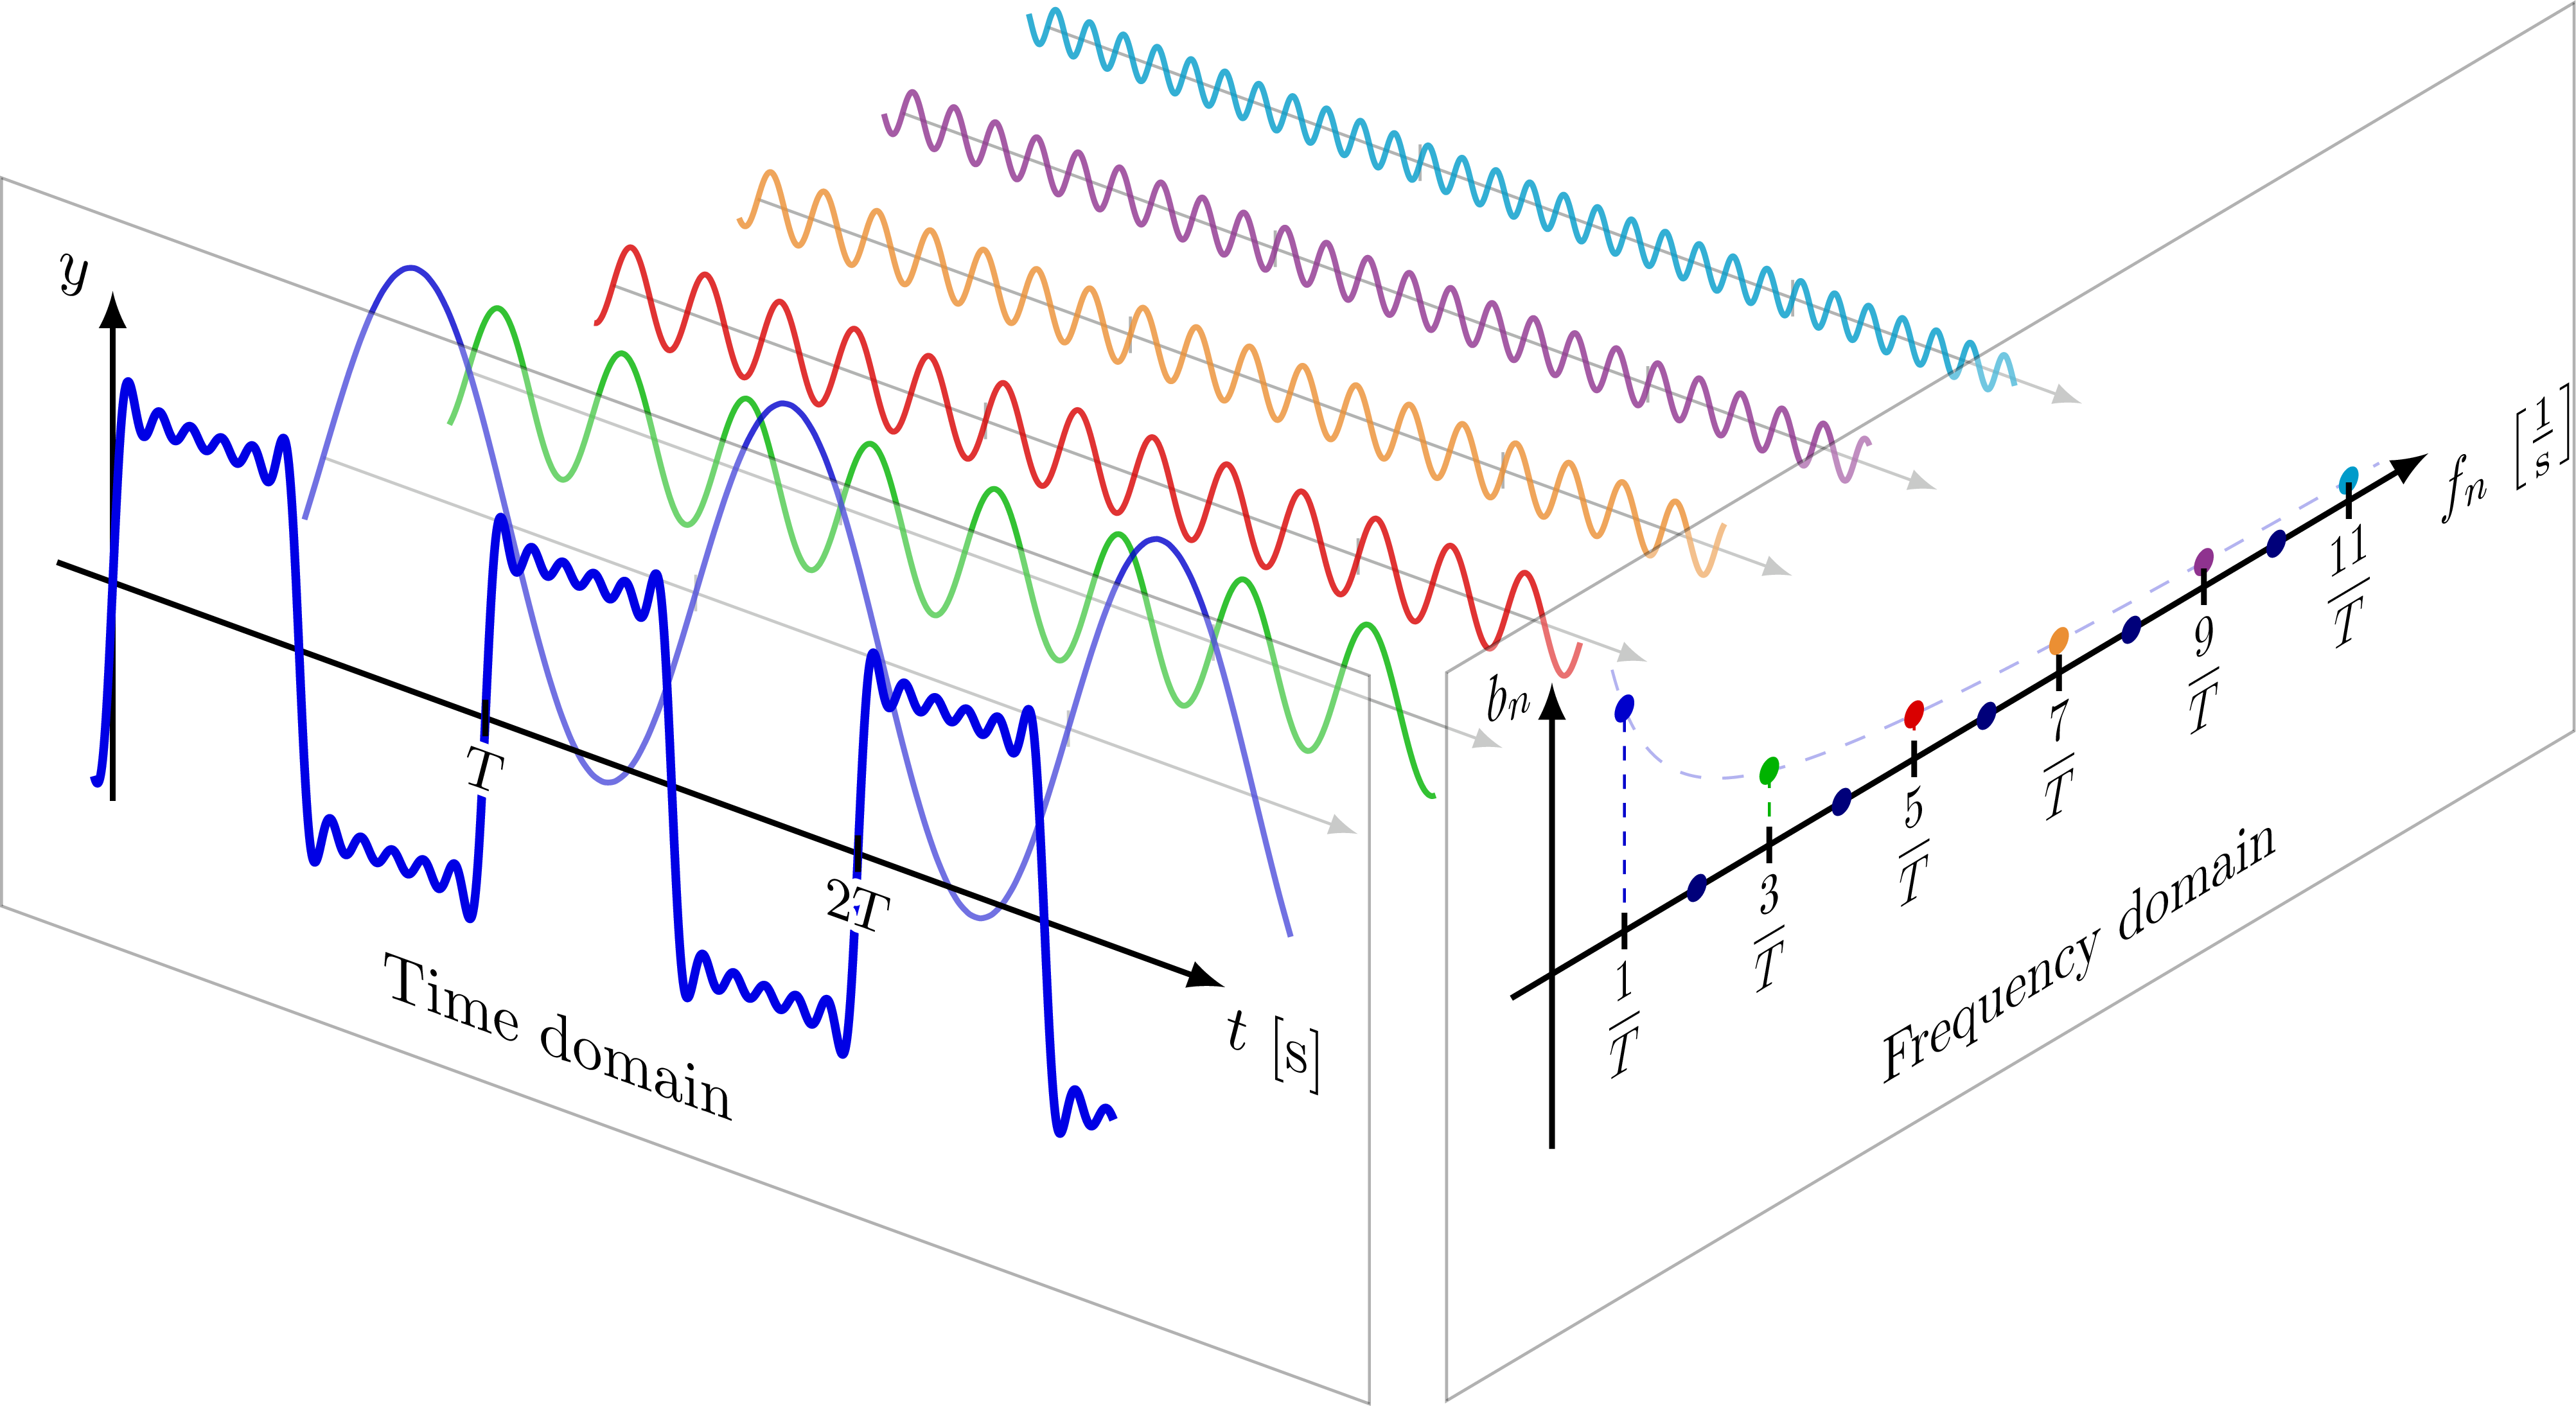
\includegraphics[width=0.5\linewidth]{Images/fourier_decomposition.png}
    \caption{Fourier Transform of a Wave$^{(1)}$}
    \label{fig:enter-label}
\end{figure}

\section*{Fourier Transform: Why?}
Now onto the "why". Why is the Fourier Transform useful? Why is it so synonymous with many industrial fields?
The answer is that the ability to analyze a waveform into pure frequencies is nearly indispensable in many fields.
\newline \newline
Take for example our application at hand: Image Compression.

\section*{Image Compression}
Image compression is the act of compressing an image (i.e: reducing its storage size) as the cost of fidelity.
Essentially, the file's size is decreased as a result of removing data stored within the image. That data is usually
the "fine details" of an image; the features of the image which give it its sharp look. Usually, image compression is split
into 5 stages

\subsection*{Stage 1: Converting the Image into a Color Matrix}
Any colored image can be represented as a matrix of RGB values, otherwise known as "color channels".
They are the essence of the image, and they are what make the image colorful and vibrant. Those three 
channels essentially comprise everything that is about a colored image. By decoding the image into those 
three channels, we can then proceed onto the analysis required to "compress" an image. 

\subsection*{Stage 2: Fourier Transforming the Color Matrix}
Here is where the Fourier Transform comes in. We Fourier Transform the image's color matrix
to obtain a matrix of color frequencies. The transformed matrix then passes onto the next stages

\subsection*{Stage 3: The Compression Process}
This process is the most essential step of the compression process; the core of the algorithm. 
Here, data is excised according to its "importance"; essentially, some of the data is removed 
while the rest is kept as is. Usually, an associated number is assigned in order to quantify 
how much data is lost. In this paper, we call it the "Compression Factor". It is given by

\begin{center}
C = \% of Data to Remove
\end{center}

However, in the compression process, a related number is most often used: the "Keep Factor"

\begin{center}
    K = 1 - C = \% of Data to Keep
\end{center}

In essence, the compression process is comprised of removing the least significant Fourier coefficients
from the Fourier transformed color matrix. The bottom $C$\% of coefficients are set to zero, while the 
top $K$\% of coefficients are left untouched.

\subsection*{Stage 4: Inverse Fourier Transforming the Color Matrix}
Here, the modified color matrix is inverse Fourier-Transformed, yielding a new color matrix which 
represents the modified image's matrix. The image has now been compressed, and is ready for the final stages

\subsection*{Stage 5: Converting the Color Matrix Into an Image}
Here, the modified color matrix is written back onto an image file. Expectedly, the image file
will be reduced in size, and the quality of the image will drop (depending on the compression factor,
the image will exhibit varying ranges of compression, usually embodied in the form of loss of crispness and
color vibrance).

\newpage
\subsection*{Results}
\begin{figure}[h]
 \begin{subfigure}[b]{0.4\textwidth}
    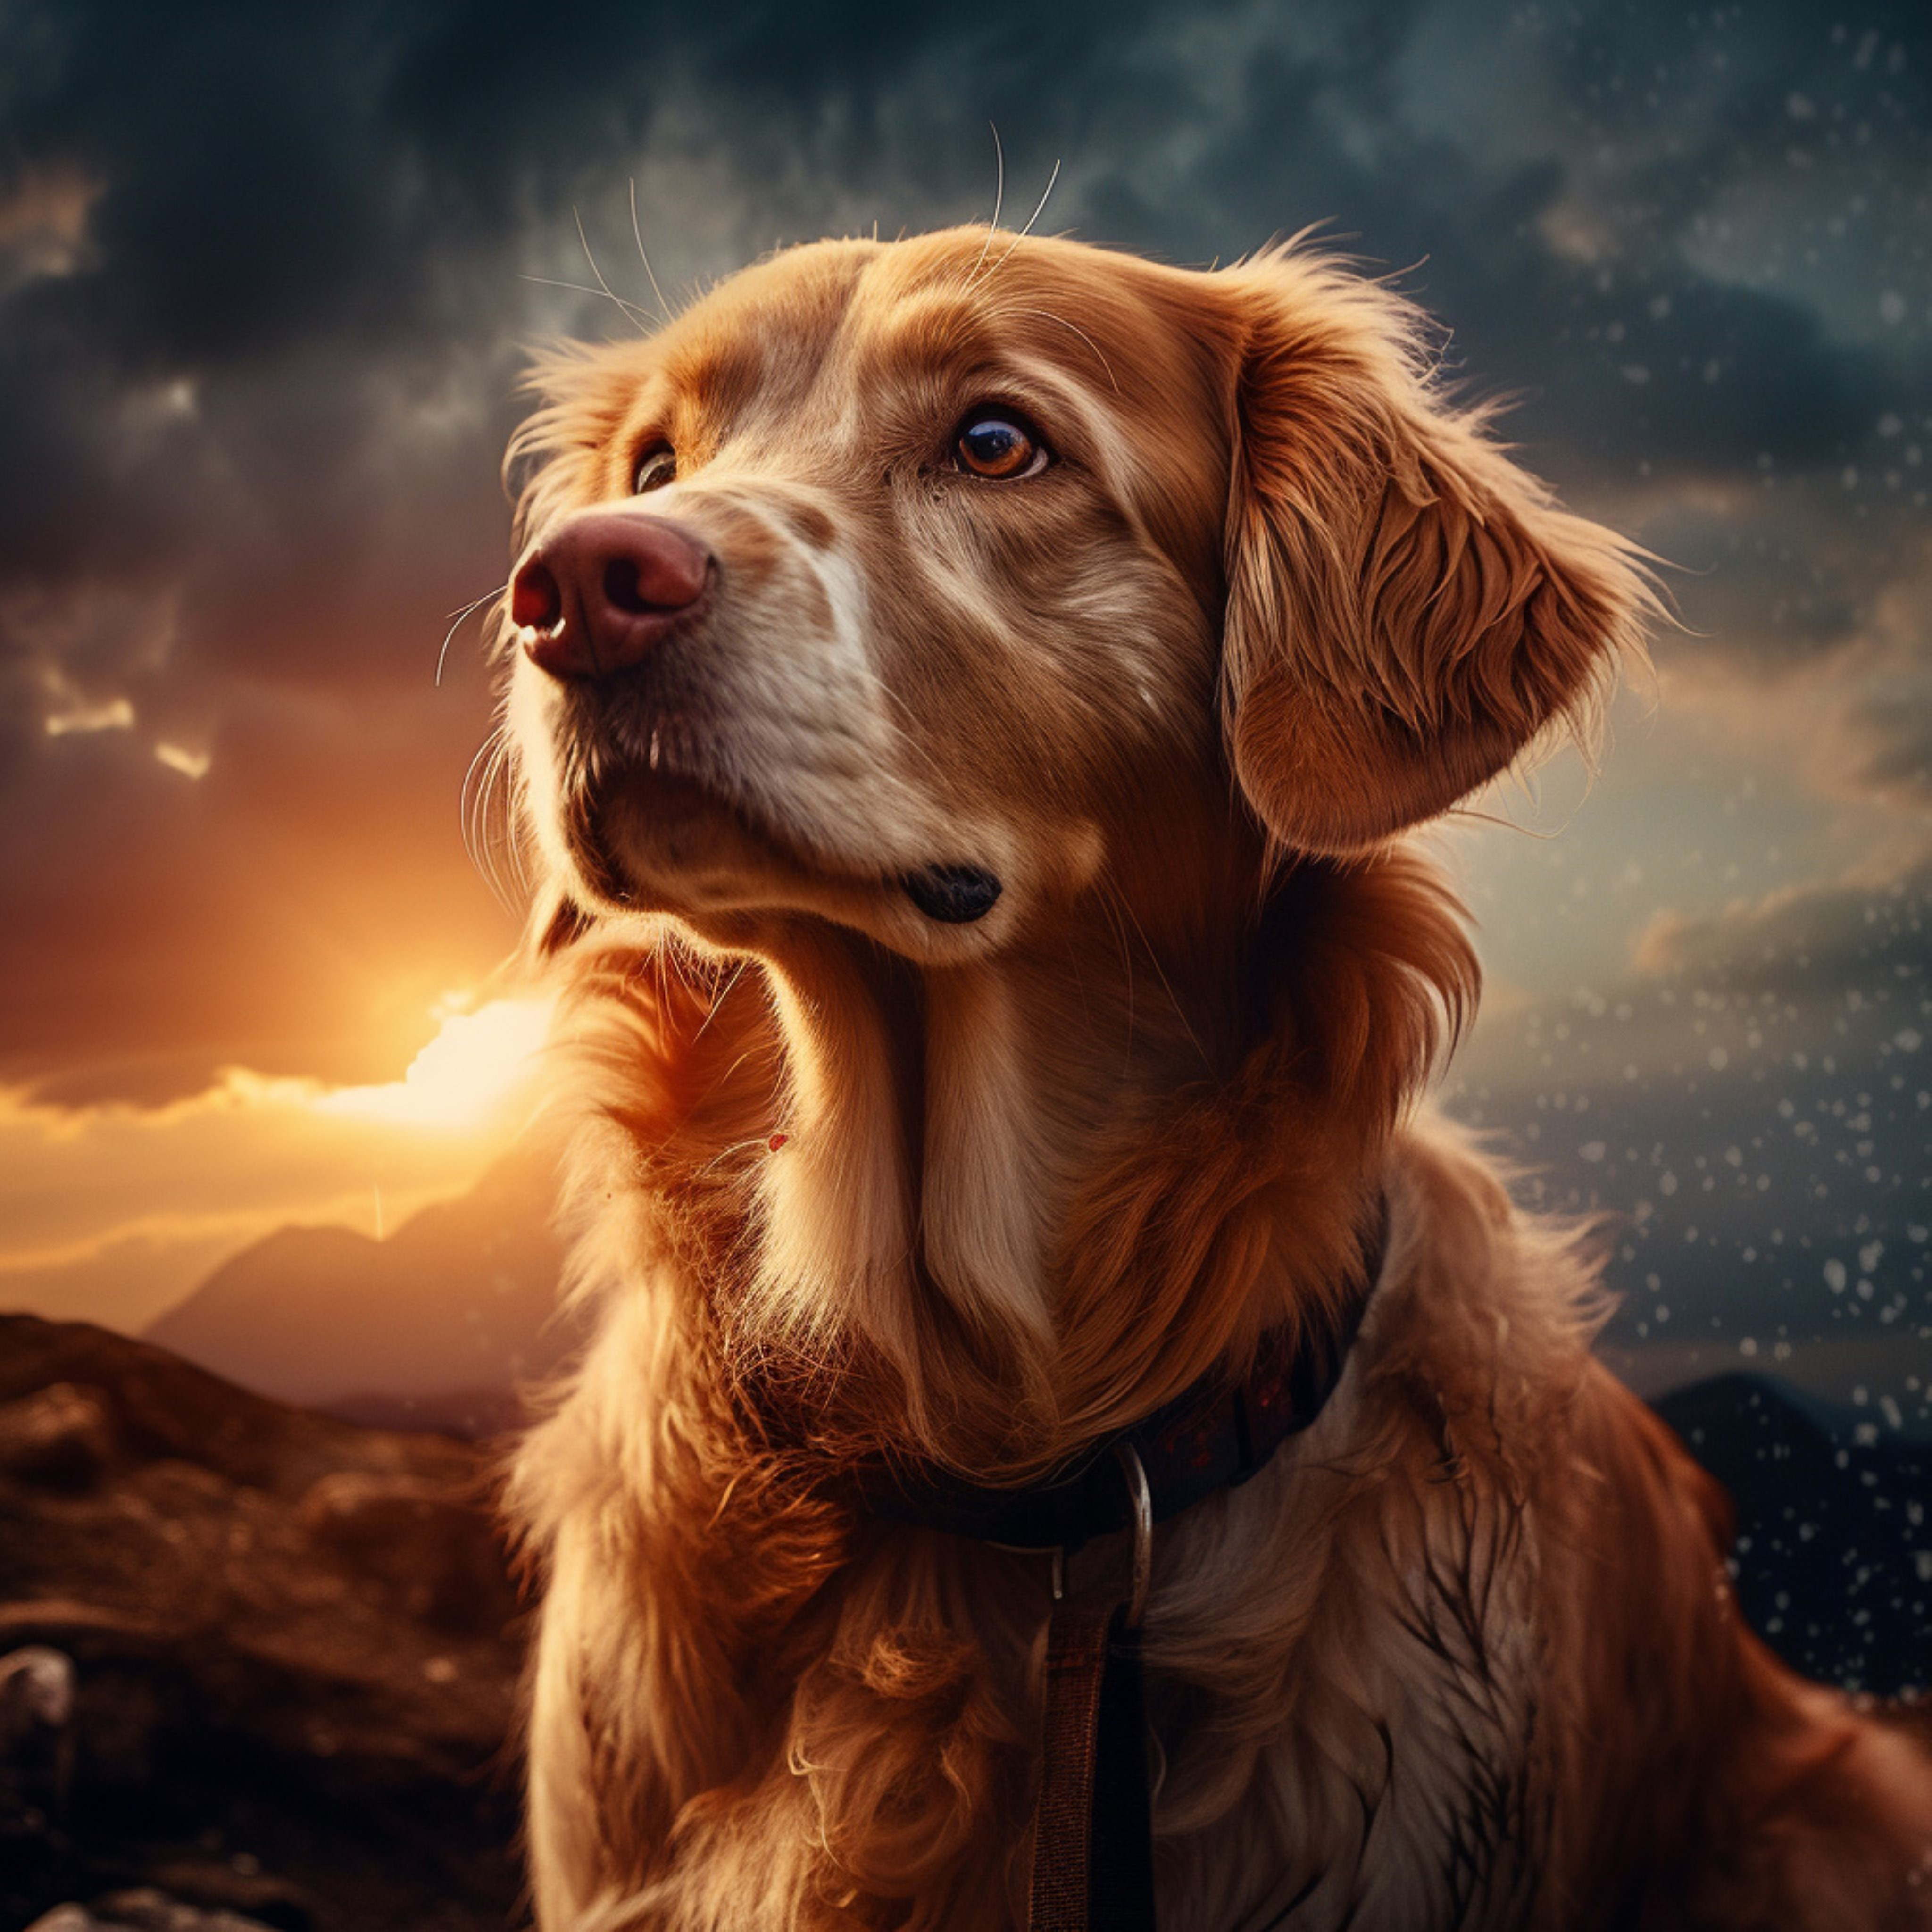
\includegraphics[width=\textwidth]{Images/uncompressed-image.jpg}
    \caption{Uncompressed (K = 1): 13.7 MB}
    \label{fig:f1}
 \end{subfigure}
 \hfill
 \begin{subfigure}[b]{0.4\textwidth}
    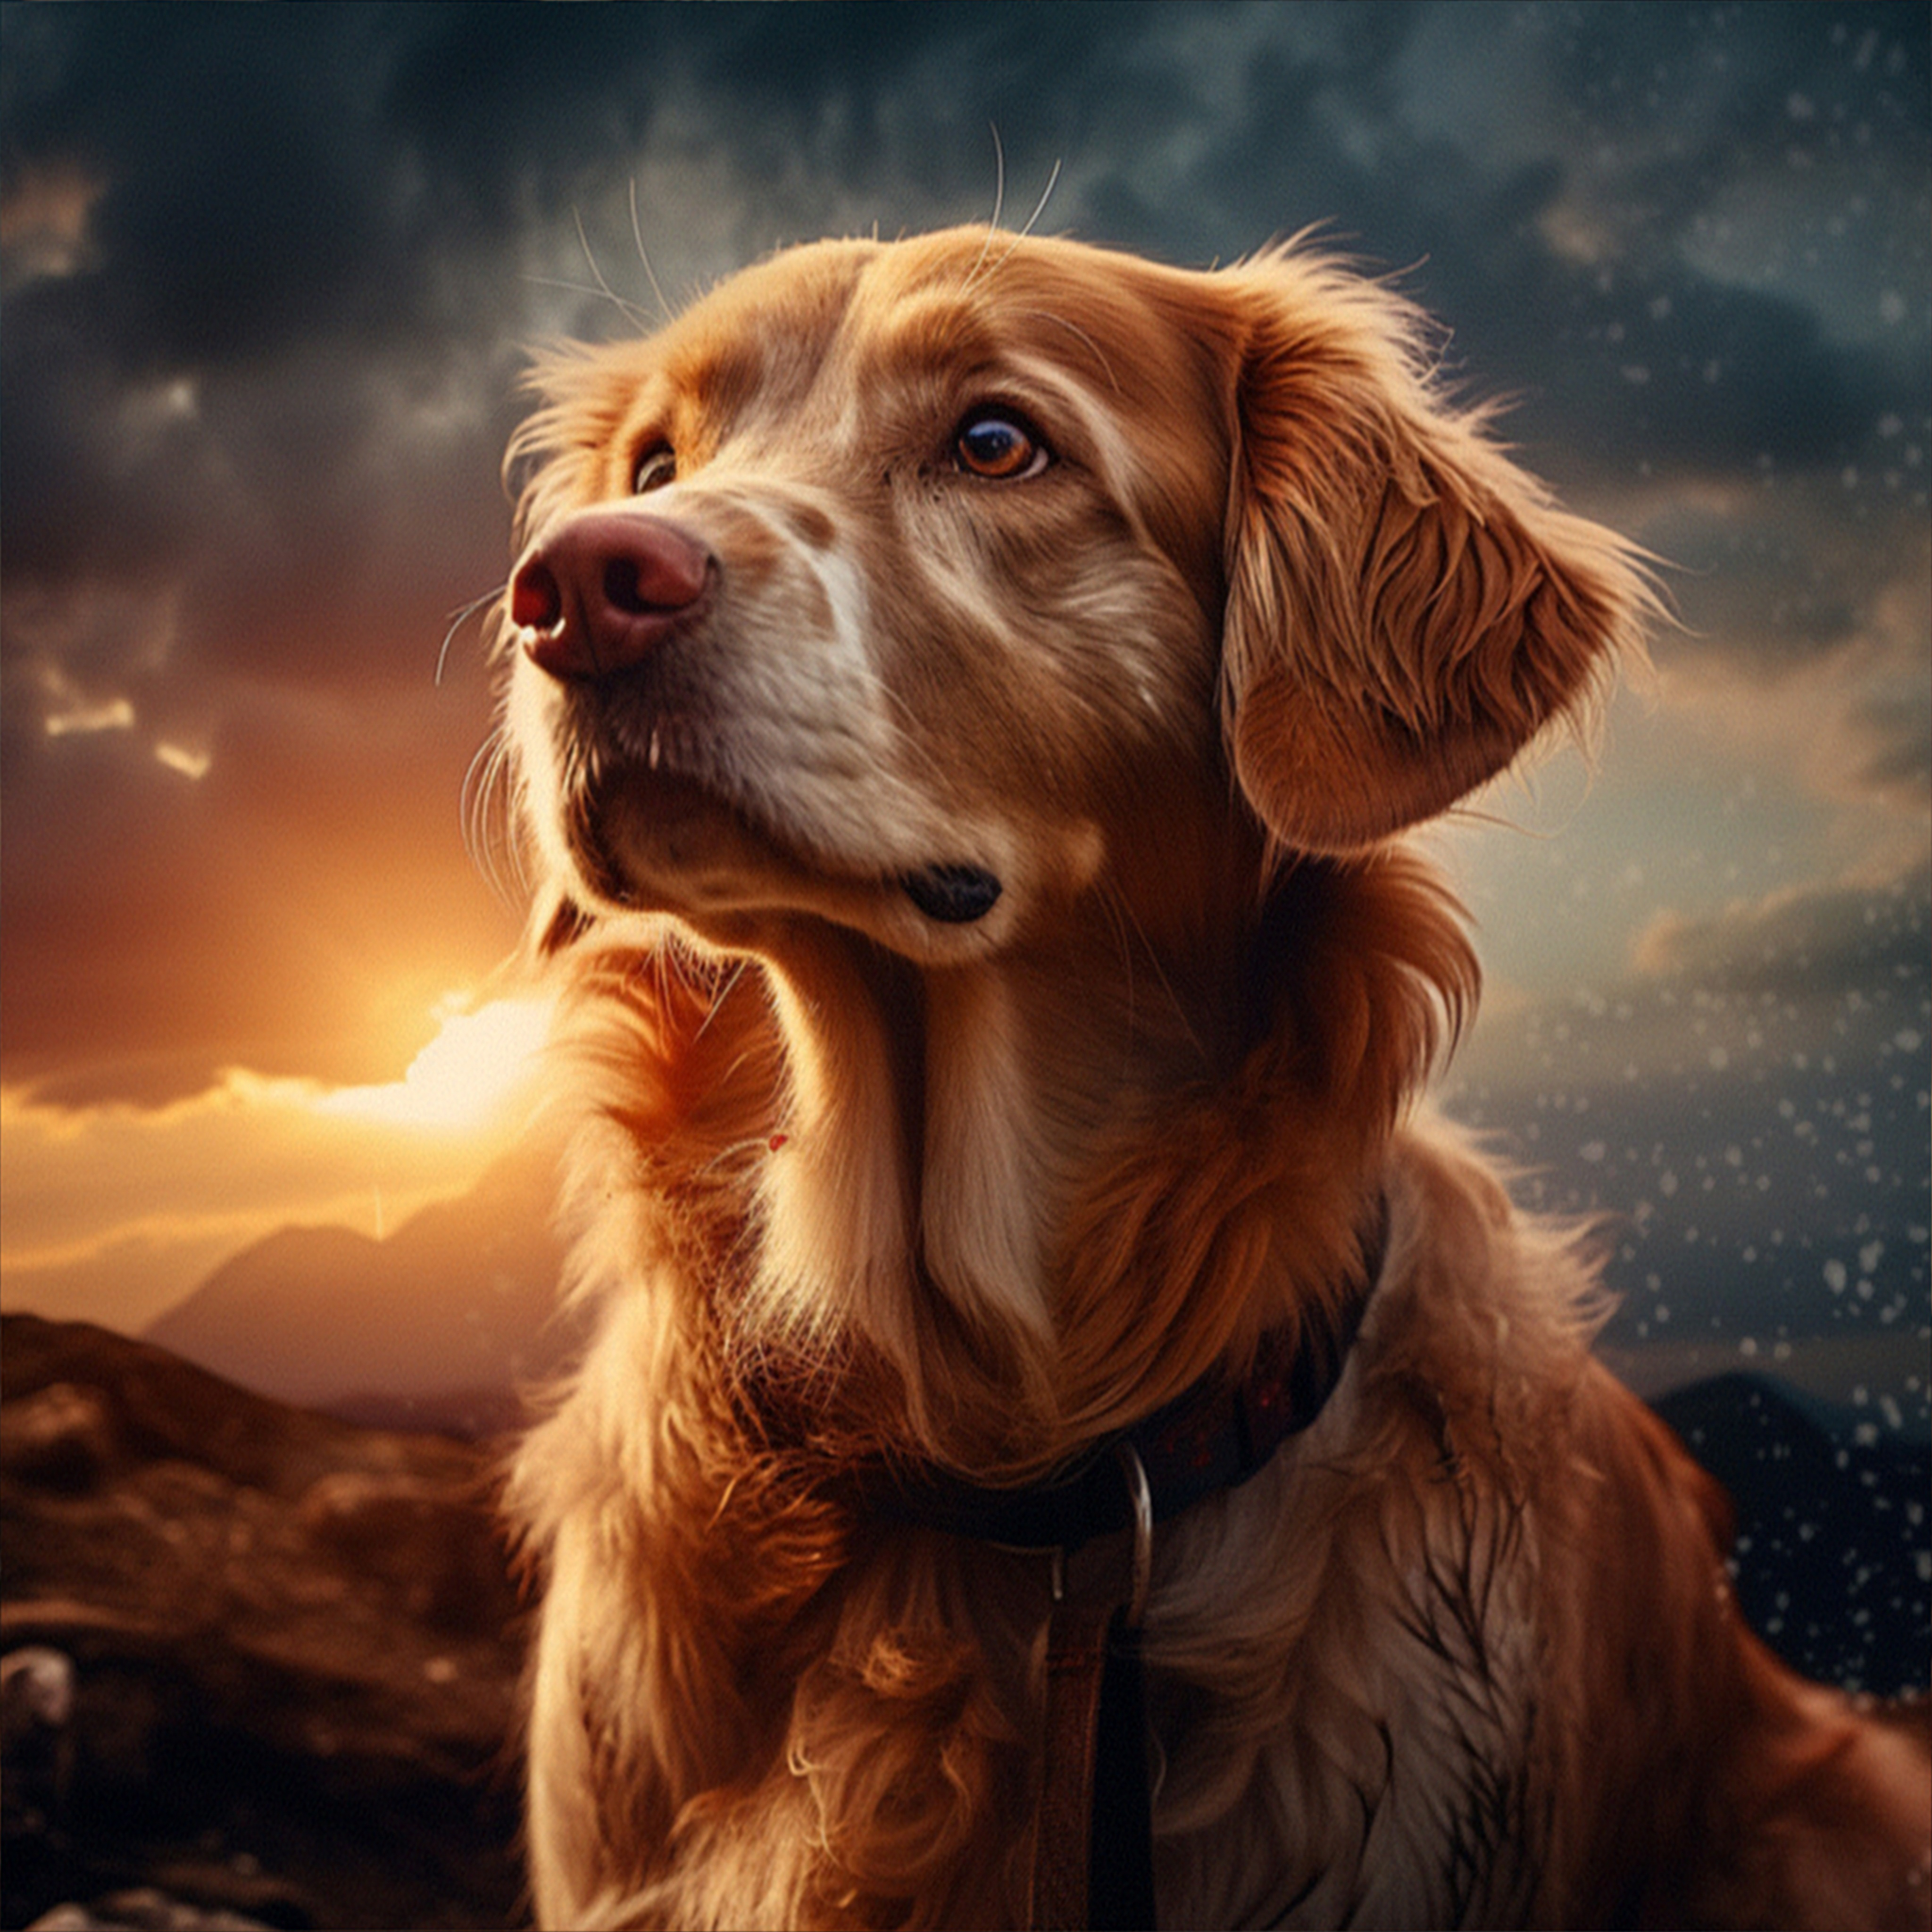
\includegraphics[width=\textwidth]{Images/compressed-image.png}
    \caption{Compressed (K = 0.01): 9.22 MB}
    \label{fig:f2}
 \end{subfigure}
 \caption{Compression Algorithm Applied to An Image }
\end{figure}
The results seem promising. However, what if we want to go further?

\begin{figure}[h]
    \centering
    \includegraphics[width=0.5\linewidth]{Images/supercompressed-image.png}
    \caption{Further Compressed Image (K = 0.004): 7.25 MB}
    \label{fig:scd}
\end{figure}
Evidently, the Fourier tranform is powerful in image compression. However, the image was spoiled, with artifacts all over, 
just for a $\approx 1.9$ times size reduction. Can we do better?

\newpage
\section*{Chapter 2: The Wavelet Transform}
The Wavelet transform is yet again another transform (just like the Fourier Transform). Its origin is attributed to many,
from Jean Morlet, to George Zweig in 1975. It decomposes signals into sums of contractions, dilations, and translations of a
mother function $\psi$, allowing the analysis of signals into frequencies evolving in time. In short, it is a potent tool, 
as we'll come to find out. 

\subsection*{Why Wavelet Over Fourier?}
You may be asking: "Why use the Wavelet transform over the Fourier transform?" The answer to that question is quite profound.
Firstly, Wavelet transforms project the function over an orthogonal basis of "wave packets", which are short bursts
of waves localized in time, with finite energy. (For further reading, please refer to $^{(2)}$).
\begin{figure}[h]
    \centering
    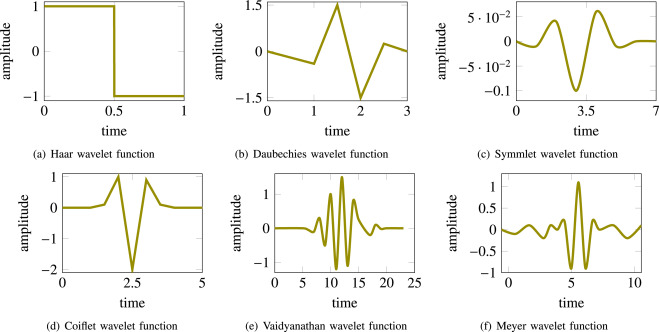
\includegraphics[width=0.5\linewidth]{Images/wavelet-types.jpg}
    \caption{Different Variants of Wavelets$^{(3)}$}
    \label{fig:wavelets}
\end{figure}
\newline
The main reason why Wavelet transforms are so powerful is due to the fact that real-life signals are 
chaotic, noisy, and irregular. Decomposing such signals into weighted sums of periodic function may work
just fine, but is not the most efficient route. As a matter of fact, the localized nature of Wavelets
allows them to represent such functions with better resolution than the standard Fourier transform.
As such, we will demonstrate the true power of the Wavelet transform shortly.

\subsection*{Image Compression Using Wavelets}
The image compression process is much the same as the Fourier tranform process. However, one stage differs slightly
\subsubsection*{Stage 1.5: Splitting the Color Channels}
The human eye responds differently to different colors on the spectrum. Further, images usually do not have identical
data in each channel (or else the image would be pure white or black!) As such, the color channels need to be split
into 3 channels (Red, Green, Blue) and each should be analyzed differently.

\subsection*{Results}
\begin{figure}[h]
    \begin{subfigure}[b]{0.4\textwidth}
       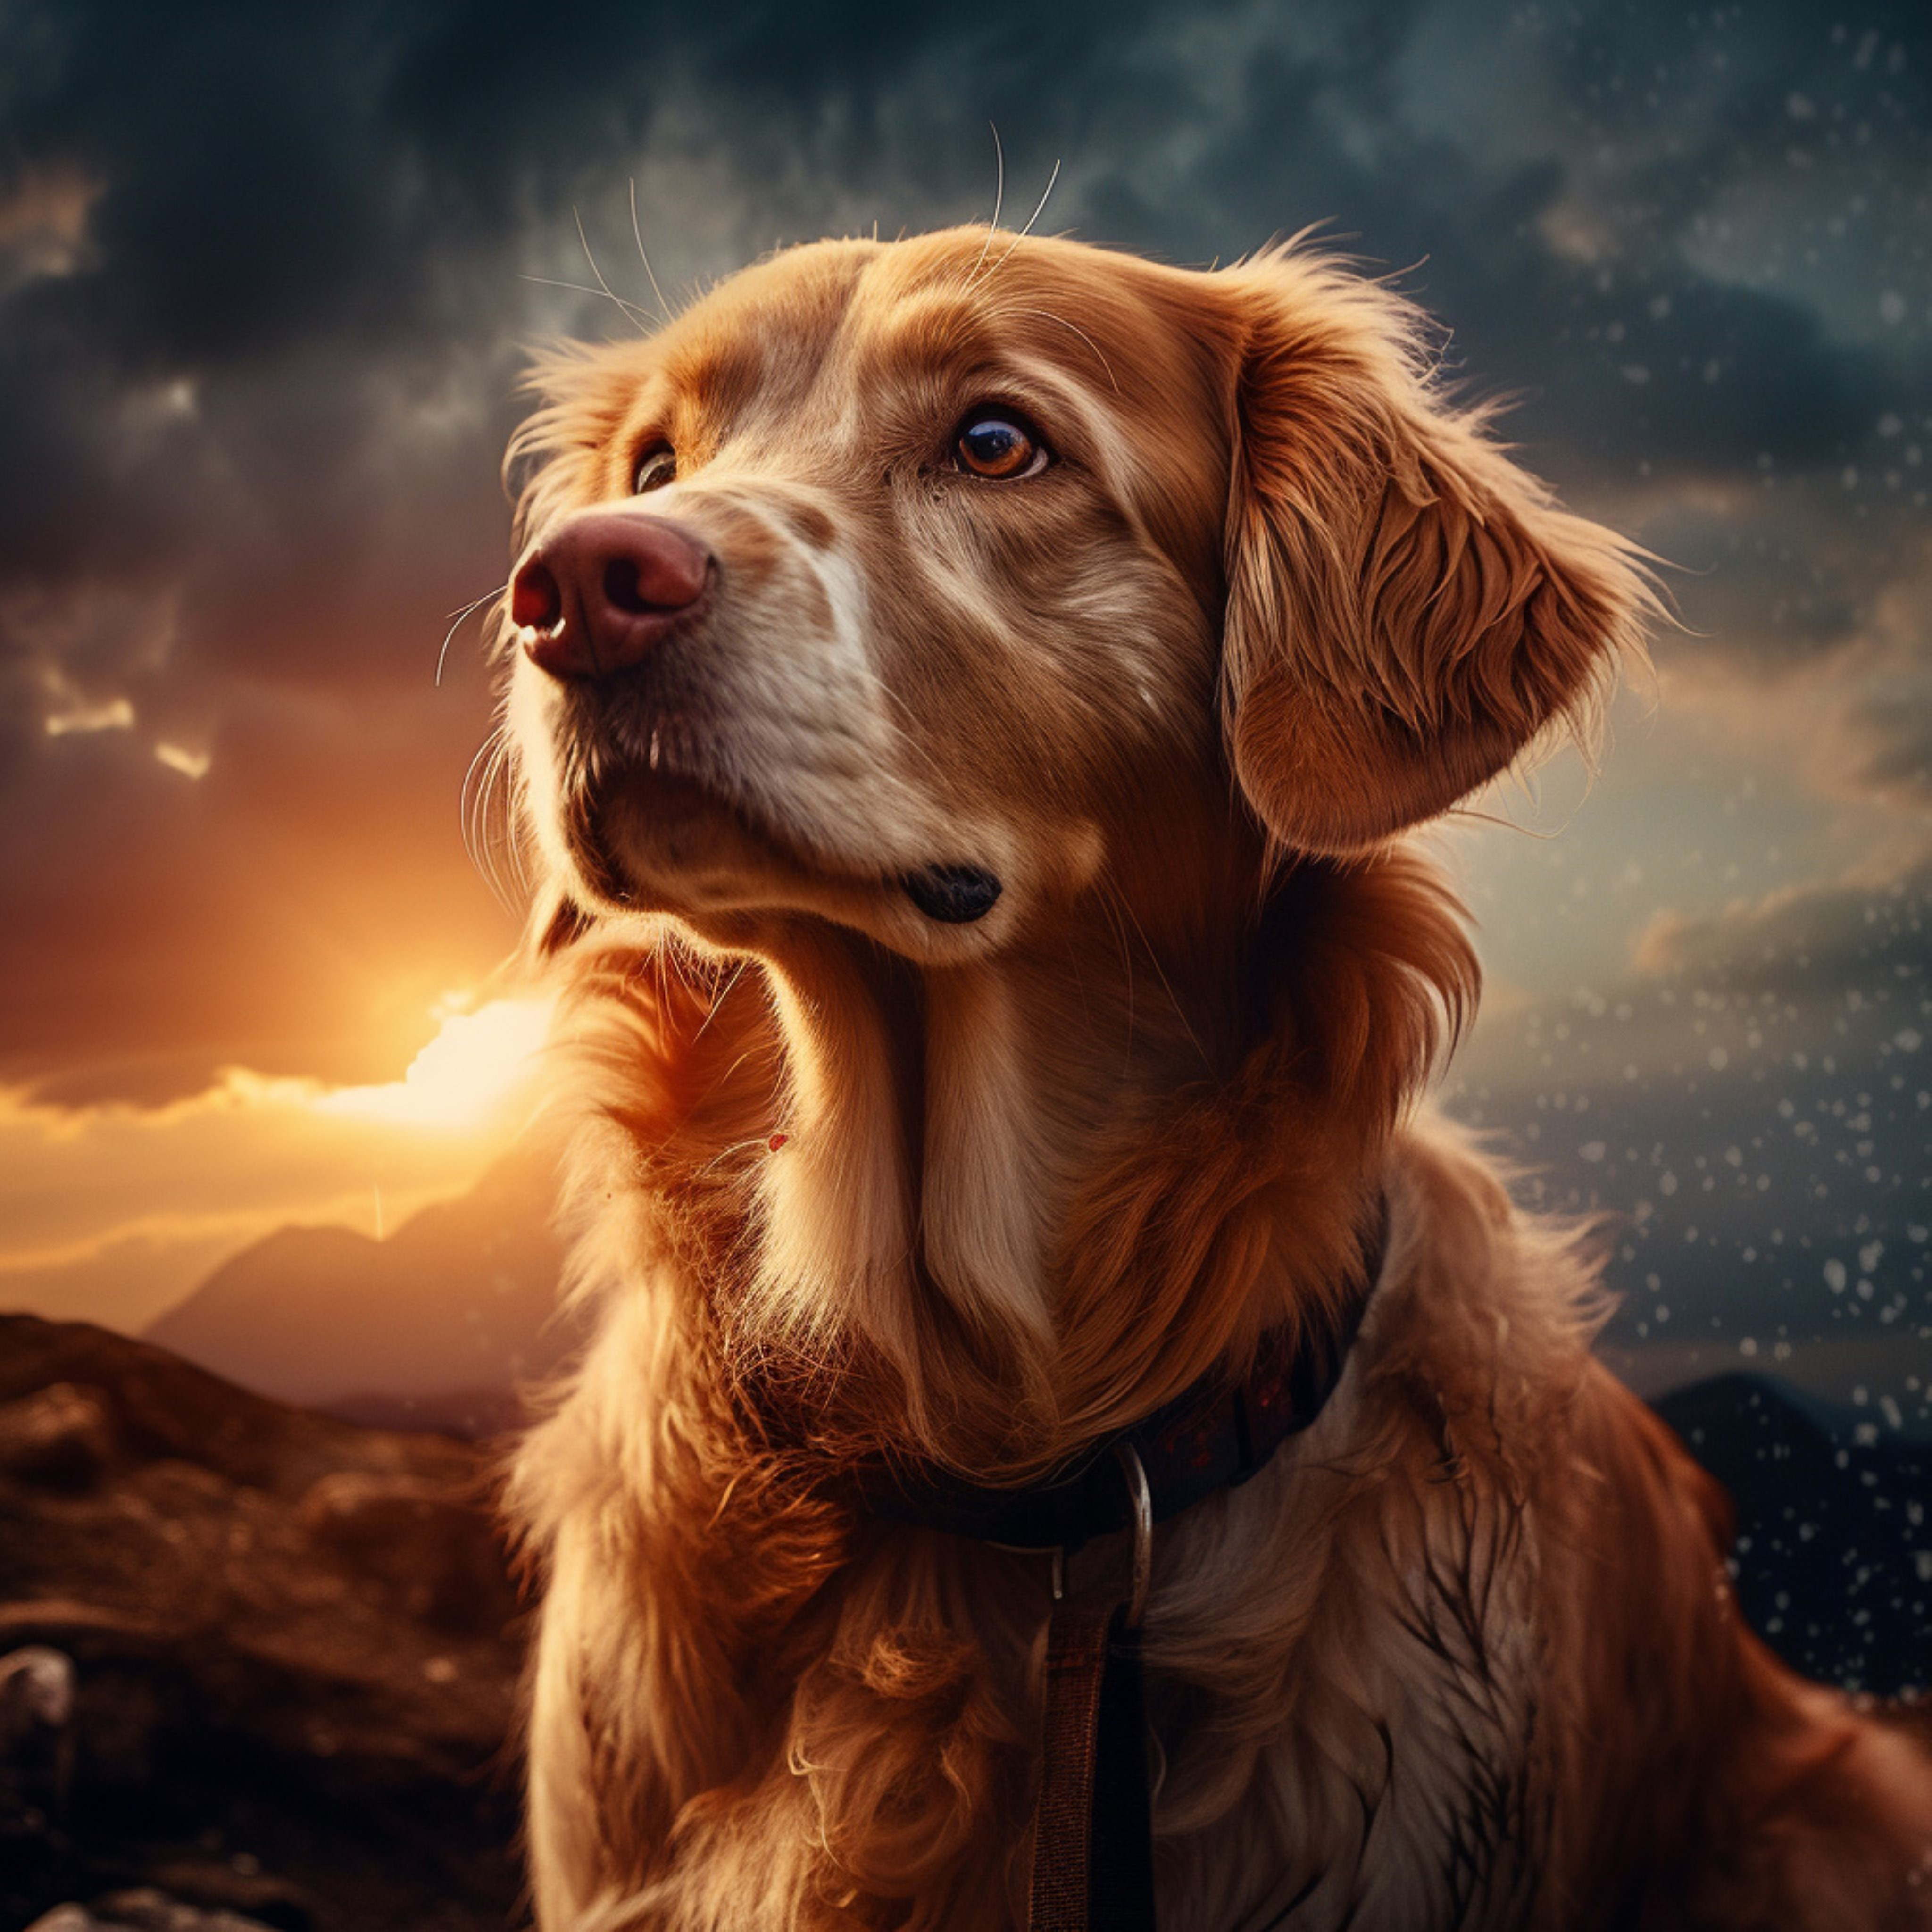
\includegraphics[width=\textwidth]{Images/uncompressed-image.jpg}
       \caption{Uncompressed (K = 1): 13.7 MB}
       \label{fig:f3}
    \end{subfigure}
    \hfill
    \begin{subfigure}[b]{0.4\textwidth}
       \includegraphics[width=\textwidth]{Images/wavelet-compressed-image.png}
       \caption{Compressed (K = 0.01): 5.05 MB}
       \label{fig:f4}
    \end{subfigure}
    \caption{Wavelet Compression Algorithm Applied to An Image }
   \end{figure}

Already, this is a remarkable increase in efficiency! We have reduced the image size by $\approx 2.7$ times with barely noticeable 
loss of fidelity! Let's go further
\begin{figure}[h]
    \centering
    
\includegraphics[width=0.5\linewidth]{Images/wavelet-supercompressed-image.png}
    \caption{Further Compressed Image (K = 0.004): 3.12 MB}
    \label{fig:scwd}
\end{figure}
\newline
Evidently, the image no longer has the artifacts present in the Fourier tranformed case. Further, it has been 
reduced in size from the corresponding Fourier transform compression by $\approx 2.3$ times!

\newpage
\section*{Conclusion}
Evidently, both the Fourier and Wavelet transforms are quite powerful means of compressing images in a lossy manner. 
However, the Wavelet transform provides better results for the same keep (K) ratios, both in fidelity and image size.
This is because the Wavelets used are comprised of short bursts of energy which are localized in time, which better
approximate a signal that is as chaotic and messy as real signals are. For this cause, Wavelet transforms are considered
extremely powerful, and are used almost routinely in image compression algorithms.

\newpage
\section*{References}
$^{(1)}$ \href{https://dibsmethodsmeetings.github.io/fourier-transforms/}{Decomposing Fourier transforms — an introduction to time-frequency decomposition}
\newline \newline
$^{(2)}$ Zhang, D., \& Zhang, D. (2019). Wavelet transform. Fundamentals of image data mining: Analysis, Features, Classification and Retrieval, 35-44.
\newline \newline
$^{(3)}$ Guido, R. C. (2022). Wavelets behind the scenes: Practical aspects, insights, and perspectives. Physics Reports, 985, 1-23.
\end{document}